\chapter{DNA sequencing}

\label{kap:dna_sequencing} % id kapitoly pre prikaz ref

Genetic information is coded in DNA (deoxyribonucleic acid) composed of two chains that coil around
each other to form a double helix. The two DNA strands are also known as polynucleotides as they are
composed of simpler monomeric units called nucleotides. Each nucleotide is composed of one of four
nitrogen-containing nucleobases (cytosine [$C$], guanine [$G$], adenine [$A$] or thymine [$T$]).

The process of figuring out the order of nucleotides in polynucleotides is called DNA sequencing.
Technologies and algorithms for DNA sequencing have been known since 70s and they are still
evolving. One of the latest methods of sequencing is the nanoporous DNA sequencing.

\section{Nanoporous DNA sequencing using MinION}

Nanopore sequencing is a unique, scalable technology that enables direct, real-time analysis of long
DNA or RNA fragments. It works by monitoring changes to an electrical current as nucleic acids are
passed through a protein nanopore. The resulting signal is decoded to provide the specific DNA or
RNA sequence.

MinION is a new real-time sequencing technology developed by Oxford Nanopore
Technologies. It is based on nanopores and it is highly portable. A nanopore is a hole so small,
that only single DNA strand fits in. MinION uses a protein nanopore set in an electrically resistant
polymer membrane. An ionic current is passed through the nanopore by setting a voltage across this
membrane. If an analyte passes through the pore or near its aperture, this event creates a
characteristic disruption in the current. Measurement of that current makes it possible to identify
the molecule in question \cite{first_look_minion}.

\begin{figure}[H]
  \centerline{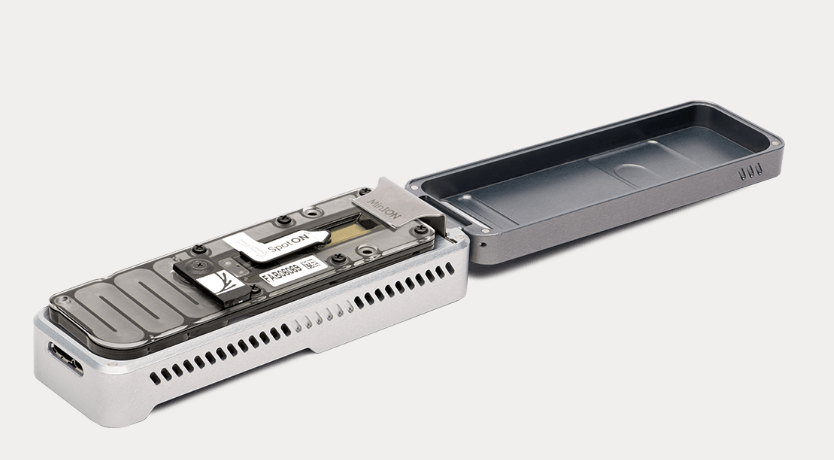
\includegraphics[width=0.8\textwidth]{images/minion}}
  \caption[MinION]{MinION - Portable DNA sequencer}
  \label{obr:minion}
\end{figure}

The electric current is measured 4000 times per second (about 10 measurments per nucleobases).
Measured values are stored in \textit{.fast5} file. This data is called \textit{raw signal}.

The process of translating current measures into a sequence of bases (letters A, C, G, T) is called
basecalling.

\subsection{Raw signal normalization}

Raw signal depends not only on the DNA sequence in the nanopore, but also other factors which may
depend in multiple reads. The raw signal therefore needs to be normalized. One of such methods in
median normalization proposed by Stoiber et. al. \cite{batmendijn_bakalarka}

\subsection{Signal conversion to nucleobases}

The normalized signal is then translated into nucleobases. Nucleobase value is depenant also by $k$
consecutive nucleobases, called \textit{K-mers}. 

There are multiple existing translators, but the translation is a slow process usually based on
hidden Markov model or recurrent neural networks. \cite{barbora_bakalarka}
